\documentclass[11pt,fleqn]{article}
\usepackage{../cs188,latexsym,epsf, amsmath,amsfonts,graphicx,url}
\lecture{6}
\def\title{Note \the\lecturenumber}
\begin{document}
\maketitle


\iffalse
\documentclass[11pt,fleqn]{article}
\usepackage{latexsym,epsf,amsmath,amsfonts,graphicx,url}

\title{Note 6}

\newcommand{\F}{\mathbb{F}}
\newcommand{\Z}{\mathbb{Z}}
\newcommand{\Q}{\mathbb{Q}}
\newcommand{\R}{\mathbb{R}}
\newcommand{\C}{\mathbb{C}}

\begin{document}

\maketitle
\fi

\section*{Probabilistic Inference}

In artificial intelligence, we often want to model the relationships between various nondeterministic events. If the weather predicts a 40\% chance of rain, should I carry my umbrella? How many scoops of ice cream should I get if the more scoops I get, the more likely I am to drop it all? If there was an accident 15 minutes ago on the freeway on my route to Oracle Arena to watch the Warriors' game, should I leave now or in 30 minutes? All of these questions (and innumerable more) can be answered with \textbf{Probabilistic Inference}.

We're assuming that you've learned the foundations of probability in CS70, so these notes will not review basic concepts of probability like PDFs, conditional probabilities, independence, and conditional independence.

In previous sections of this class, we modeled the world as existing in a specific state that is always known. For the next several weeks, we will instead use a new model where each possible state for the universe has its own probability. For example, we might build a weather model, where the state consists of the season, temperature and weather. Our model might say that $P(winter, 35^\circ, cloudy) = 0.00023$. This number represents the probability of the specific outcome that it is winter, 35 degrees, and cloudy.

More precisely, our model is a \textbf{joint distribution}, i.e. a table of probabilities which captures the likelihood of each possible \textbf{outcome}, also known as an \textbf{assignment}. As an example, consider the table below:


\begin{center}	
	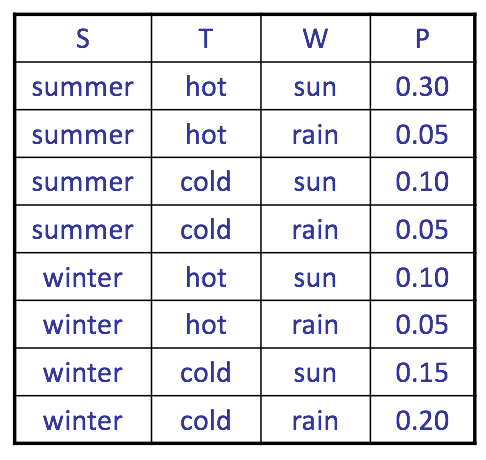
\includegraphics[width=10cm]{img/pdf_example}
\end{center}

This model allows us to answer questions that might be of interest to us, for example:

\begin{itemize}
\item What is the probability that it is sunny? $P(w = sunny)$
\item What is the probability distribution for the weather, given that we know it is winter? $P(W | s = winter)$
\item What is the probability that it is winter, given that we know it is rainy and cold? $P(s = winter | t = cold, w = rain)$
\end{itemize}

Given a joint PDF, we can trivially perform compute any desired probablity $P(Q|e_1...e_k)$ using a simple intuitive procedure known as \textbf{Inference by Enumeration}. In this procedure, we collect all the rows consistent with the evidence available (i.e. $e_1...e_k$, sum out all the hidden variables (i.e. all variables for which we do not have evidence), and finally normalize the table so that it is a probability distribution.

For example, if we wanted to compute $P(W | s = winter)$, we'd select the four rows where s is winter, we'd sum out the 



\section*{Bayes Nets (Representation)}

Naturally, representing an entire joint distribution in the memory of a computer is not very scalable - if each of $n$ variable we wish to represent can take on $d$ possible values (it has a \textbf{domain} of size $d$), then our joint distribution table will have $d^n$ entries! 

Bayes nets avoid this issue by taking advantage of the idea of conditional probability. Rather than storing information in a giant table, it is instead distributed across a large number of smaller local probability tables along with a \textbf{directed acyclic graph} which captures the relationships between variables. 

Specifically, each node in the graph represents a single random variable. Arrows in the graph represent conditional independent relationships. A node is conditionally independent of its ancestors given all of its parents. Thus, if we have a node representing variable Q, we store $P(Q | X_1, X_2, ..., X_N)$, where $X_1, ..., X_N$ are the parents of Q.

As an example of a Bayes Net, consider a model where we have five binary random variables described below:

\begin{itemize}
\item B: Burglary occurs.
\item A: Alarm goes off.
\item E: Earthquake occurs.
\item J: John calls.
\item M: Mary calls.
\end{itemize}

Assume the alarm can go off if either a burglary or an earthquake occurs, and that Mary and John will call if they hear the alarm. In this case, we can represent the natural conditional independences with the graph shown below.

\begin{center}	
	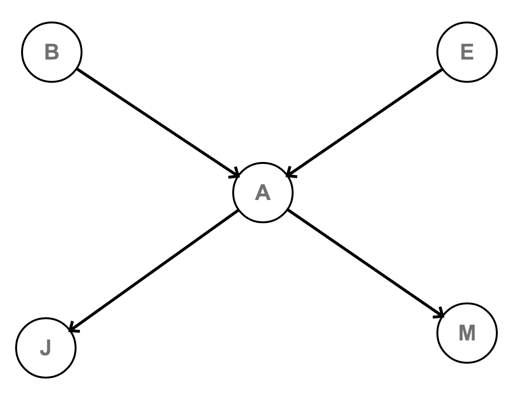
\includegraphics[width=10cm]{img/alarm_model}
\end{center}

Models capture a way the world works - they are always a simplification - key
all models are wrong, but some will still be useful for solving real problems in the real world. They may may not account for every variable or even every interaction between variables.

\section*{Representation}

More formally, we say that a Bayes Net consists of:
\begin{itemize}
\item A directed acyclic graph of nodes, one per variable X.
\item A conditional distribution for each node $P(X | A_1 ... A_n)$, where $A_i$ is the ith parent of X, stored as a \textbf{conditional probability table} or CPT.
\end{itemize}

Given all of the CPTs for a graph, we can calculate the probability of a given assignment using the chain rule: $P(x_1, x_2, ..., x_n) = \prod_{i=1}^n{x_i | parents(X_i)}$. 

For the alarm model above, we might calculate the probability of one event as follows: $P(-b, -e, +a, +j, -m) = P(-b) \cdot P(-e) \cdot P(+a | -b, -e) \cdot P(+j | +a) \cdot P(-m | +a)$.

This works because of the conditional indepences given by the graph. Specifically, we rely on the fact that $P(x_i | x_1, ..., x_{i-1}) = P(x_i | parents(X_i))$. Or in other words, that the probability of a specific value of $X_i$ depends only on the values assigned to $X_i$'s parents.

While it is most natural to assign arrows in a Bayes Net in the same direction as causality, e.g. $earthquake \rightarrow alarm$, the direction of the arrows does not change the space of possible distributions represented by the Bayes Net. That is, if you flip an arrow, it is possible to pick new values for the CPTs such that the joint distribution is unchanged. Or stated differently: Our model is ultimately a joint distribution over all variables. The direction of the arrows does not affect which values are possible in the joint table, though the absence of arrows may restrict the possible values for the joint table, e.g. if there are no arrows, the values in the joint PDF table will need to reflect the fact that all variables are independent.

\section*{Inference}

Inference is the process of calculating the joint PDF for some set of query variables based on some set of observed variables. We can solve this problem naively by forming the joint PDF and using Inference by Enumeration. This requires creation and iteration over an exponentially large table.

An alternate approach is to \textbf{eliminate} variables one by one. To eliminate a variable X, we: 

\begin{itemize}
\item Join (multiply together) all factors involving X.
\item Sum out X.
\end{itemize}

For example, suppose we have a model as shown below, where T, C, S, and E can take on binary values, as shown below:

\begin{center}	
	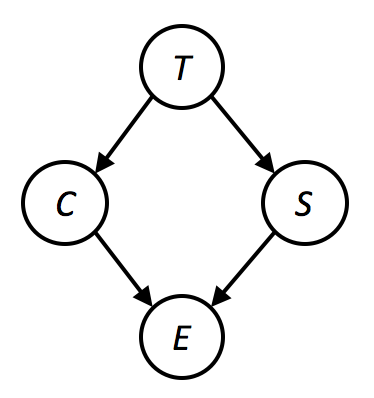
\includegraphics[width=10cm]{img/TCSE_model.png}
\end{center}

In this case, we have the factors $P(T)$, $P(C|T)$, $P(S|T)$, and $P(E|C, S)$. Suppose we want to calculate $P(T | +e)$. The naive approach would be to form the 16 row joint PDF $P(T, C, S, E)$, select only the rows corresponding to +e, then summing out C and S and finally normalizing. 

The alternate approach is to eliminate C, then S, one variable at a time.

Suppose we eliminate C first. In this case, we'd join (multiply) all the factors involving C, namely $P(C|T)$ and $P(+e|C, S)$. The product rule tells us that this product equals $P(C, +e | T, S)$. We'd then sum out C, leaving us with a new factor $P(+e | T, S)$. 

At this point, we now have three factors $P(T)$, $P(S|T)$, and our new factor $P(+e | T, S)$. To eliminate S, we'd join (multiply) $P(S|T)$ and $P(+e | T, S)$, yielding $P(+e, S | T)$. Summing over S we'd get $P(+e | T)$.

With S and T eliminated, we are left with two factors: $P(T)$ and $P(+e | T)$. Recall that our goal is to calculate $P(T | +e)$. To calculate this, we multiply our two factors, yielding $P(+e, T)$. Finally, we normalize, yielding $P(T|+e)$.

While this process is more involved from a conceptual point of view, the maximum size of any factor generated is only 8 rows instead of 16 as it would be if we formed the entire joint PDF.

An alternate way of looking at the problem is to observe that the calculation of $P(+e, T)$ can either be done, as it is in Inference by Enumeration, as follows:

$\sum_s{\sum_c{P(T)P(s|T)P(c|T)P(+e|c,s)}}$

Variable elimination is equivalent to calculating $P(+e, T)$ as follows:

$P(T)\sum_s{P(s|T)\sum_e{P(c|T)P(+e|c,s)}}$

\section*{Sampling}

An alternate approach for probabilistic reasoning

\end{document}

\textbf{Bayesian networks} (Bayes nets for short), graphical models that capture the conditional independence relationships between variables we want to represent and when done correctly can allow us to make good predictive inferences about various questions we wish to answer. Let's get started by discussing how Bayes' nets are constructed. <DONT LIKE THIS MAKE IT BETTER>

With this efficient storage, we can recompute any desired probabilities on demand by running \textbf{probabilistic inference} on the local probability distributions. 